\subsection{Packages-Applicazione Bring-It}
\label{Architettura ad alto livello-BringIt}
\begin{figure}[H]
	\centering
	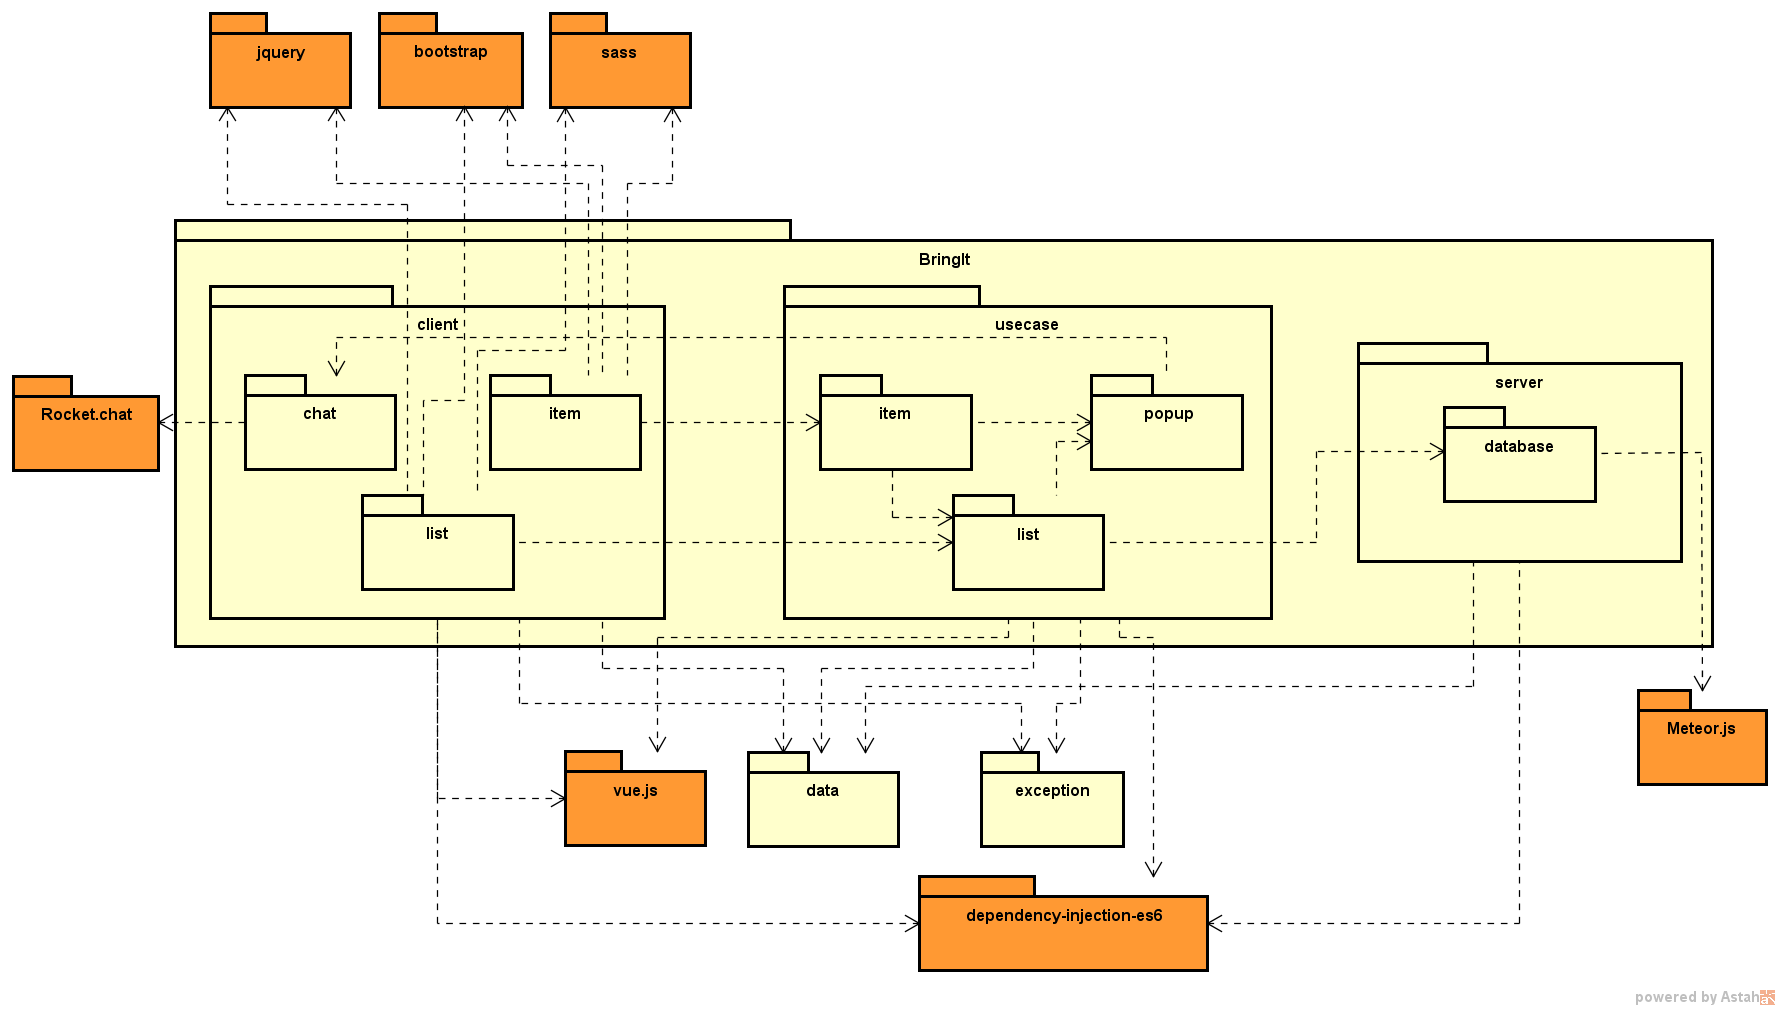
\includegraphics[width=\textwidth]{Sezioni/Packages/App/pck_application.png}
	\caption{Architettura ad alto livello Bring-It}
\end{figure}
\begin{itemize}

	\item \textbf{Descrizione}: architettura ad alto livello dell’applicazione \textit{Bring-It} del gruppo \gruppo. Data la natura dell'applicazione, si è scelto di utilizzare il \termine{pattern architetturale} Model-View-Presenter. Le funzionalità sono state divise secondo lo schema classico di un progetto Meteor: lato client, lato server e la parte che gestisce la comunicazione per le altre due. Il lato client si occupa dell'interazione con l'utente, ovvero conterrà tutte quelle componenti che reagiranno alle varie azioni che egli compie e tali cambiamenti saranno visibili all'utente tramite la chat di \termine{Rocket.Chat}. La parte server invece comunicherà direttamente con il \termine{DBMS}, ovvero \termine{MongoDB}, che si occuperà di salvare i dati necessari per il corretto funzionamento dell'applicativo. Si noti che per comunicare con il \termine{database} verrà utilizzata l'interfaccia che già offre Meteor.
Infine in seguito verranno elencati tutti i packages forniti di una spiegazione esaustiva sulle loro interazioni.
	\item \textbf{Classi e packages contenuti}:
	\begin{itemize}
		\item \textbf{application::client}: package contenente i packages e il codice che è necessario lato client. Ovvero tutte le \termine{View} ed i \termine{Presenter} che si occupano di prendere gli input dall'utente (View) e di gestirli (Presenter).
		\item \textbf{application::usecase}: package contenente tutti gli usecase dell'applicazione. Essi rappresentano tutti i models delle funzionalità offerte dall'applicativo, riceveranno i dati dai rispettivi \termine{presenter} e agiranno per compiere l'azione dell'utente.
		\item \textbf{application::server}: package contenente classi che interagiscono con l'interfaccia di Meteor che a sua volta comunicherà con il \termine{DBMS} \termine{MongoDB}.
		\item \textbf{application::data}: package contenente le classi che possono risultare utili sia alla parte client che alla parte server.
		\item \textbf{application::exception}: package contenente la gerarchia di eccezioni definita dal gruppo. Queste sono state inserite al fine di permettere una modellazione maggiore da parte degli sviluppatori che voglio usare l'\termine{SDK}.
	\end{itemize}
	\item \textbf{Librerie e Framework}
	\begin{itemize}
	\item \textbf{jQuery}: libreria JavaScript. Essa è stata inclusa per garantire operazioni di basso livello (come l'interazione con i nodi del documento HTML) o comunque per avere la garanzia che se qualcosa non è possibile farla con un \termine{framework}, possiamo usare jQuery.
	\item \textbf{Bootstrap}: \termine{framework} che serve per facilitare l'utilizzo del CSS con l'HTML.
	\item \textbf{Sass}: Sass è un'estensione retrocompatibile con CSS. Esso facilita molto la scrittura del CSS poiché provvisto di più funzionalità, rendendo la scrittura del file più facile. Viene utilizzato per creare fogli di stile di alcune pagine da visualizzare nel client. E' possibile caricare fogli di stile tramite Meteor.
	\item \textbf{Vue.js}: ??
	\item \textbf{Dependency-injection-es6}: libreria per Node.js e per gli ambienti di sviluppo JavaScript con Ecmascript 6. Essa è utile per \termine{Inversion of Control} e {Dependency Injection}.
	\item \textbf{Meteor}: piattaforma di sviluppo completa di molte funzionalità. Essa è fondamentale, oltre per l'ambiente di esecuzione, anche poiché fornisce l'interfaccia con MongoDB e permette l'aggiunta di pacchetti tramite \termine{Atmosphere}.
	\end{itemize}
\end{itemize}

\subsection{Package application::client}
\label{Package application::client}
\begin{figure}[H]
	\centering
	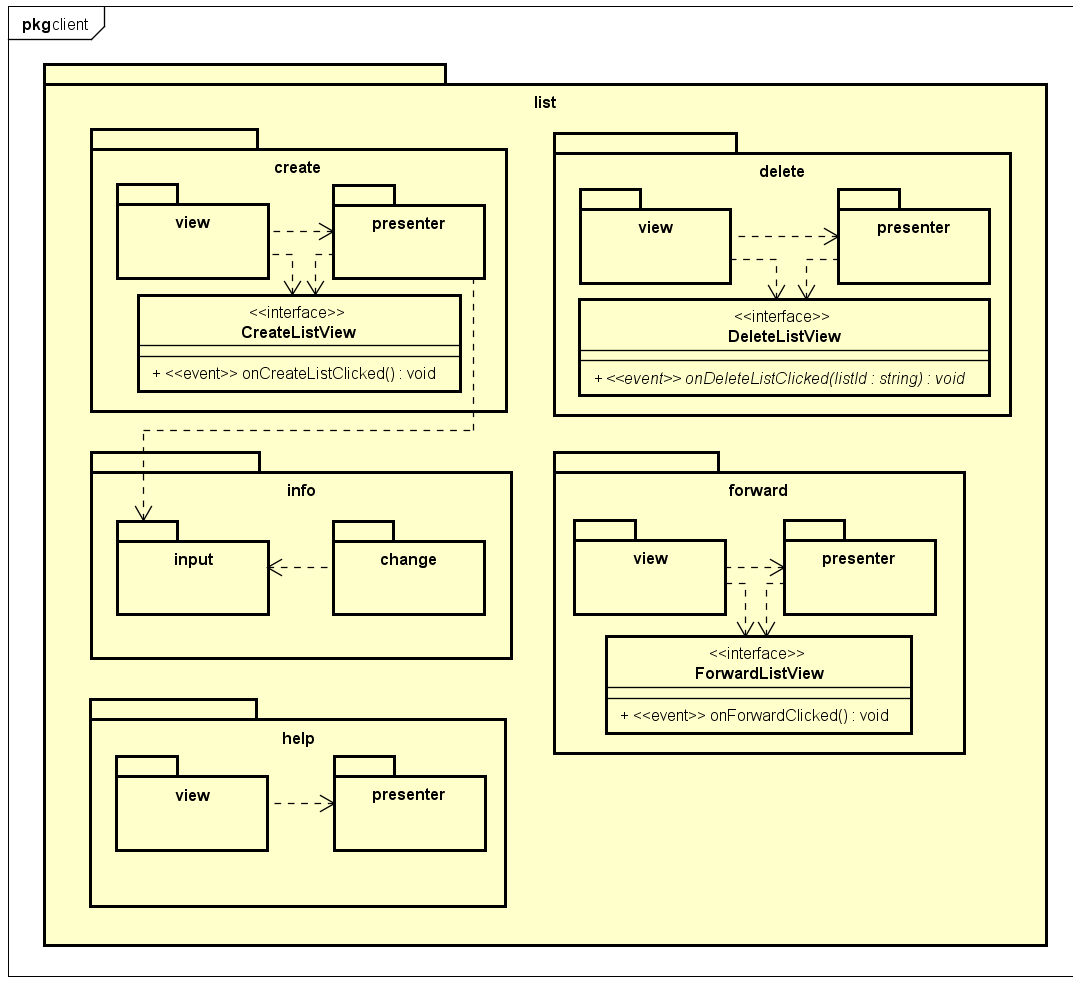
\includegraphics[width=\textwidth]{Sezioni/Packages/App/pck_client1.png}
	\caption{Package application::client-img1}
\end{figure}

\label{Package application::client}
\begin{figure}[H]
	\centering
	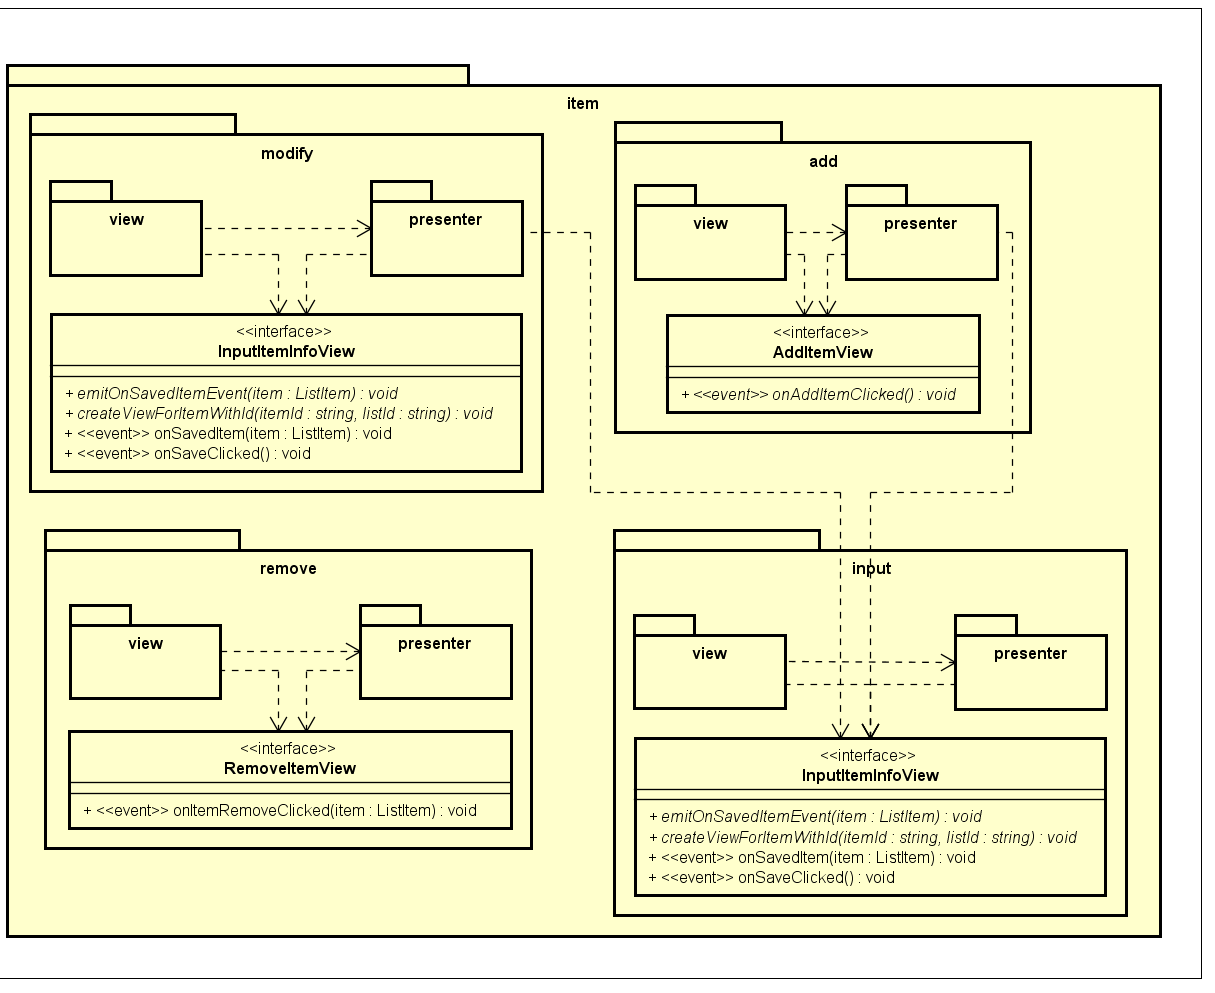
\includegraphics[width=\textwidth]{Sezioni/Packages/App/pck_client2.png}
	\caption{Package application::client-img2}
\end{figure}

\begin{itemize}
\item \textbf{Descrizione}: package contenente le componenti adibite alle funzionalità lato client. Il package chat non è stato rappresentato poiché contenente solo un'interfaccia che, una volta implementata, interagirà con la chat di \termine{Rocket.Chat} per l'invio delle bolle progettate.
\item \textbf{Classi e packages contenuti}:
\begin{itemize}
\item \textbf{application::client::list}: package contenente le componenti che rappresentano la lista che l'utente può creare.
\item \textbf{application::client::item}: package contenente le componenti che rappresentano gli elementi della lista che l'utente può aggiungere alla lista.
\end{itemize}
\end{itemize}

\subsubsection{Package application::client::list}
\label{Package application::client::list}
\begin{figure}[H]
	\centering
	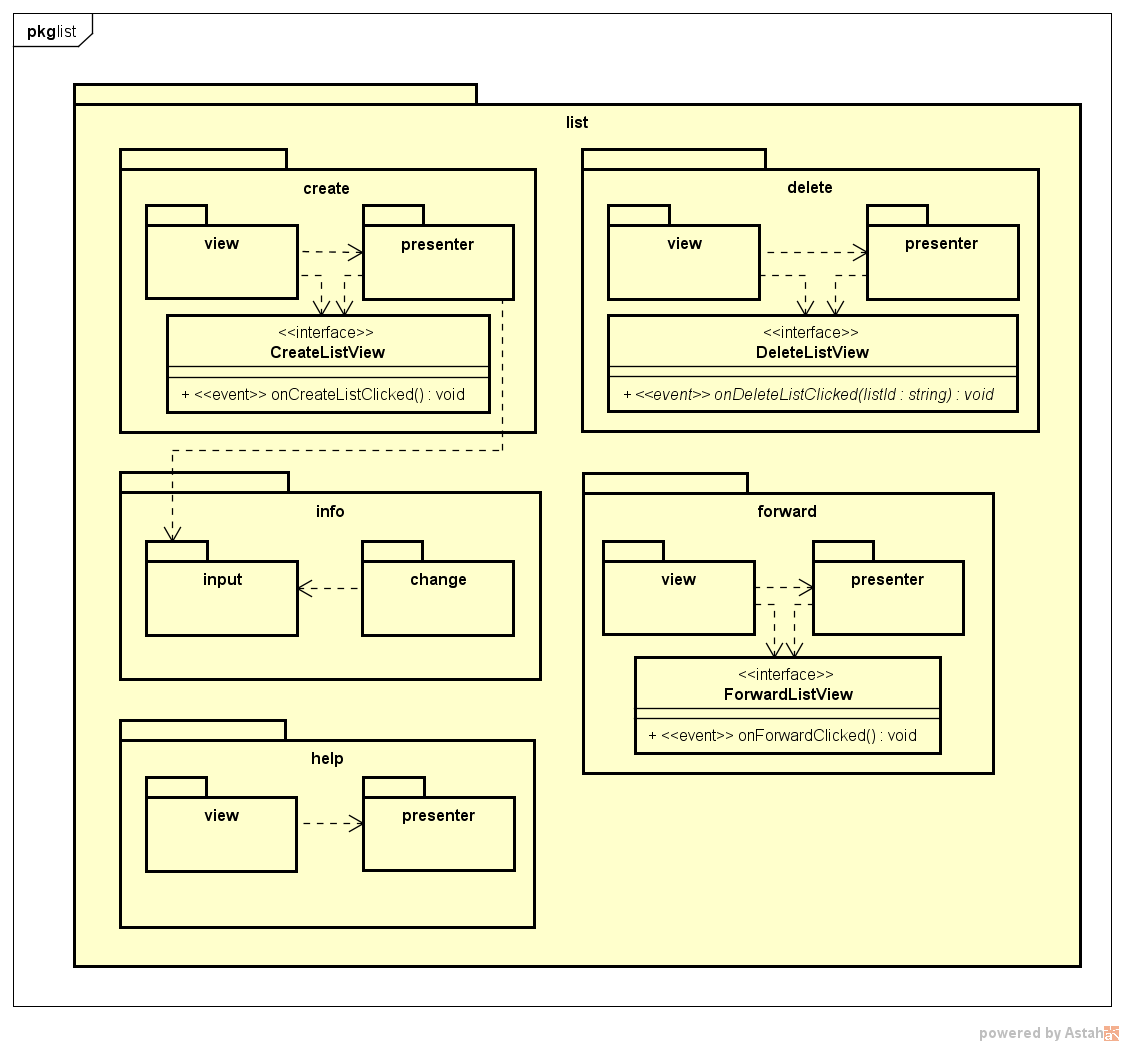
\includegraphics[scale=0.5]{Sezioni/Packages/App/pck_client_list.png}
	\caption{Package application::client::list}
\end{figure}
\begin{itemize}
\item \textbf{Descrizione}: package contenente altri package che contengono a loro volta View, \termine{Presenter} e interfaccia delle funzionalità previste per la creazione, modifica e rimozione della lista. Ogni package, dunque, conterrà la stessa struttura appena citata, perciò quelli più interni non verranno presentati poiché contenenti informazioni ridondanti e poco specifiche a rappresentare le interazioni tra le componenti. Le classi invece saranno presentate nella sezione contenente i Diagrammi delle Classi.
	\item \textbf{Classi e packages contenuti}:
	\begin{itemize}
	\item \textbf{application::client::list::create}: package che contiene le funzionalità per la creazione della lista da parte dell'utente.
	\item \textbf{application::client::list::delete}: package che contiene le funzionalità per l'eliminazione della lista da parte dell'utente.
	\item \textbf{application::client::list::info}: package che contiene le informazioni della lista creata dall'utente.
	\item \textbf{application::client::list::forward}: package che contiene le funzionalità per l'inoltro in un'altra chat della lista da parte dell'utente.
	\item \textbf{application::client::list::help}: package che contiene le le funzionalità per la richiesta di aiuto all'utilizzo della lista da parte dell'utente.
	\end{itemize}
\end{itemize}

\subsubsection{Package application::client::item}
\label{Package application::client::item}
\begin{figure}[H]
	\centering
	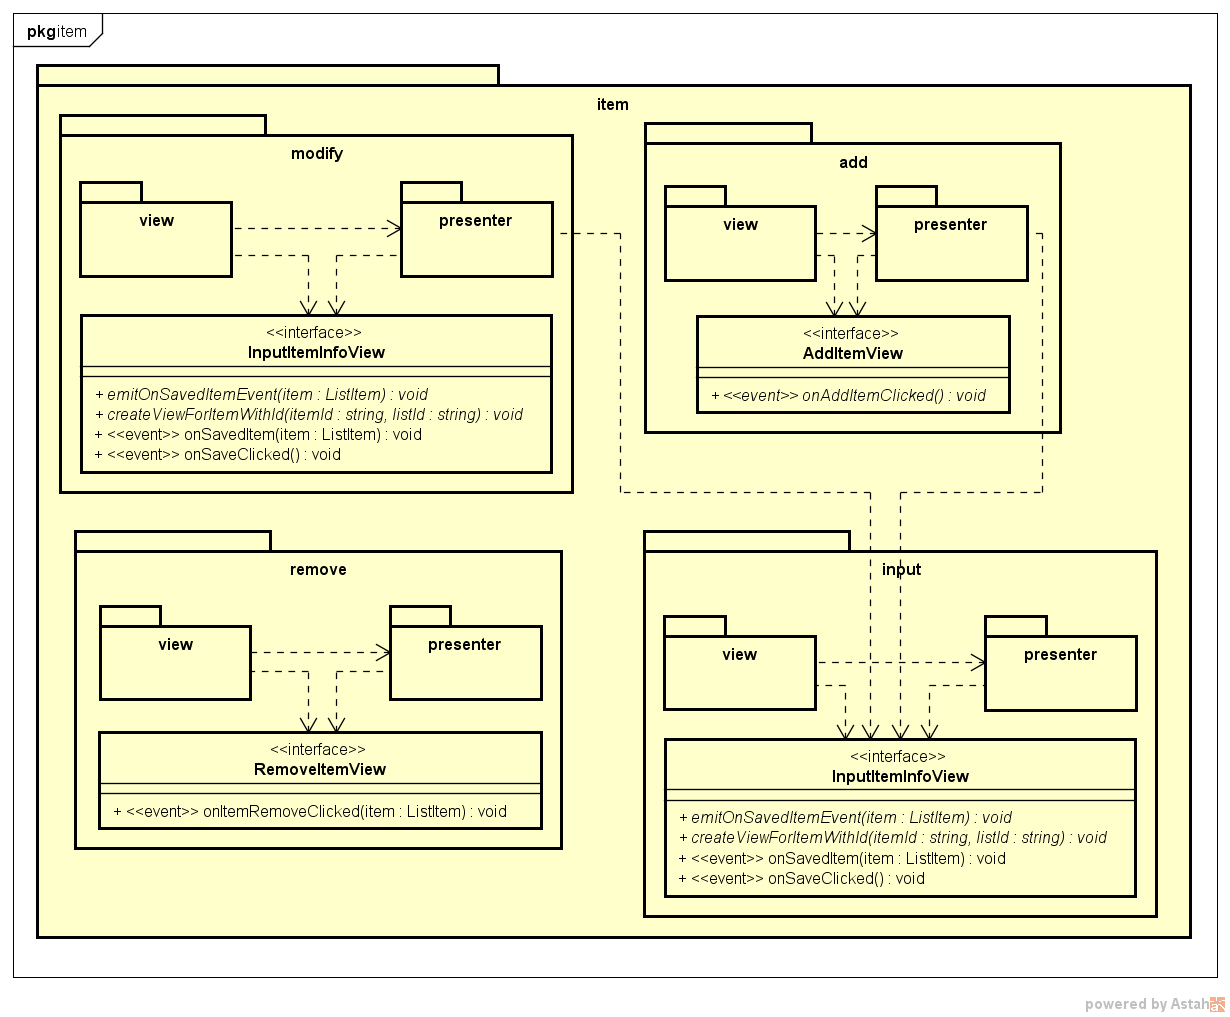
\includegraphics[scale=0.5]{Sezioni/Packages/App/pck_client_item.png}
	\caption{Package application::client::item}
\end{figure}
\begin{itemize}
	\item \textbf{Descrizione}: package contenente altri package che contengono a loro volta View, \termine{Presenter} e interfaccia delle funzionalità previste per la creazione, modifica e rimozione degli elementi della lista.
	\item \textbf{Classi e packages contenuti}:
	\begin{itemize}
	\item \textbf{application::client::item::modify}: package che contiene le componenti per garantire la modifica degli elementi o item presenti all'interno della lista.
	\item \textbf{application::client::item::remove}: package che contiene le componenti per garantire la corretta rimozione degli elementi o item presenti all'interno della lista.
	\item \textbf{application::client::item::add}: package che contiene le componenti per garantire l'aggiunta degli elementi o item presenti all'interno della lista.
	\item \textbf{application::client::item::input}: package che contiene le componenti per permettere all'utente di inserire i dati di un oggetto della lista quando va ad aggiungere un nuovo elemento o a modificarne uno già presente nella lista.
\end{itemize}
\end{itemize}

\subsection{Package application::usecase}
\label{Package application::usecase}
\begin{figure}[H]
	\centering
	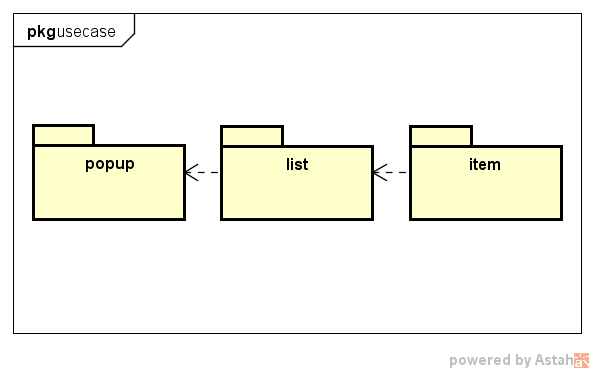
\includegraphics[scale=0.6]{Sezioni/Packages/App/pck_usecase.png}
	\caption{Package application::usecase}
\end{figure}
\begin{itemize}
\item \textbf{Descrizione}: package contenente le componenti adibite alla comunicazione tra il lato client e il lato server. In altre parole le componenti presenti in questo package rappresentano i Model delle funzionalità previste. Esse ricevono dati dal presenter e interagiscono anche con il server per svolgere correttamente le loro funzioni.
\item \textbf{Classi e packages contenuti}:
\begin{itemize}
\item \textbf{application::usecase::popup}: package che contiene le componenti logiche per l'invio dei popup che serviranno all'utente per modificare, aggiungere o rimuovere elementi dalla lista.
\item \textbf{application::usecase::list}: package che contiene le componenti logiche della lista.
\item \textbf{application::usecase::item}: package che contiene le componenti logiche degli item presenti nella lista.
\end{itemize}
\end{itemize}

\subsection{Package application::server::database}
\label{Package application::server::database}
\begin{figure}[H]
	\centering
	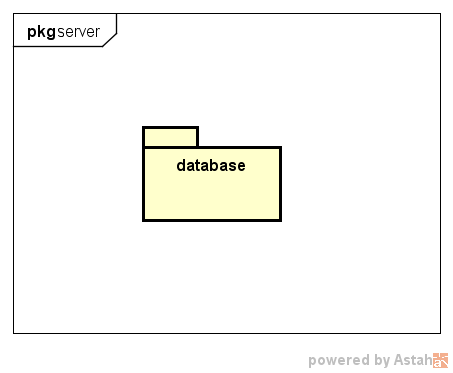
\includegraphics[scale=0.6]{Sezioni/Packages/App/pck_server.png}
	\caption{Package application::server::database}
\end{figure}

\begin{itemize}
\item \textbf{Descrizione}: questo package contiene l'interfaccia che poi implementata andrà ad interagire direttamente con l'interfaccia del database presente dentro Meteor.
\end{itemize}

















\begin{comment}

\subsubsection{Package application::communication}
\label{Package application::communication}
\begin{figure}[H]
	\centering
	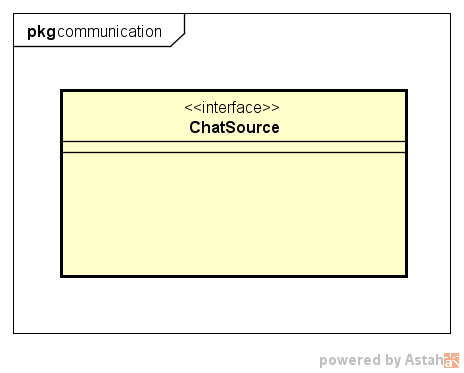
\includegraphics[scale=0.5]{Sezioni/Packages/App/communication.png}
	\caption{Package application::communication}
\end{figure}
\begin{itemize}
	\item \textbf{Descrizione}: package che contiene le classi di comunicazione con l'istanza di Rocket.chat
	\item \textbf{Classi e packages contenuti}:
	\begin{itemize}
	\item application::communication::ChatSource: interfaccia che permette la comunicazione con l'istanza di Rocket.chat
	\end{itemize}
\end{itemize}

\subsubsection{Package application::database}
\label{Package application::database}
\begin{figure}[H]
	\centering
	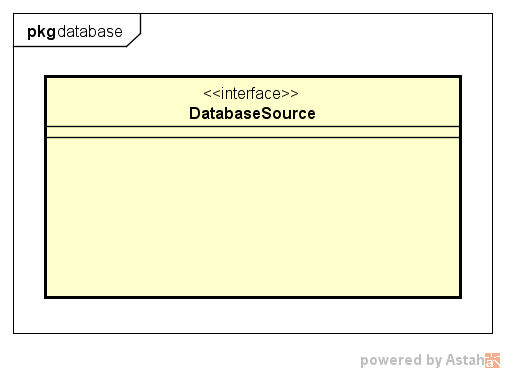
\includegraphics[scale=0.5]{Sezioni/Packages/App/database.png}
	\caption{Package application::database}
\end{figure}
\begin{itemize}
	\item \textbf{Descrizione}: package che contiene le classi per interfacciarsi con il database all'interno del quale sono salvati i dati delle liste
	\item \textbf{Classi e packages contenuti}:
	\begin{itemize}
	\item application::database::DatabaseSource: interfaccia che permette la comunicazione con il database all'interno del quale sono salvati i dati delle varie liste
	\end{itemize}
\end{itemize}

\subsubsection{Package application::feature::add\_item}
\label{Package application::feature::add_item}
\begin{figure}[H]
	\centering
	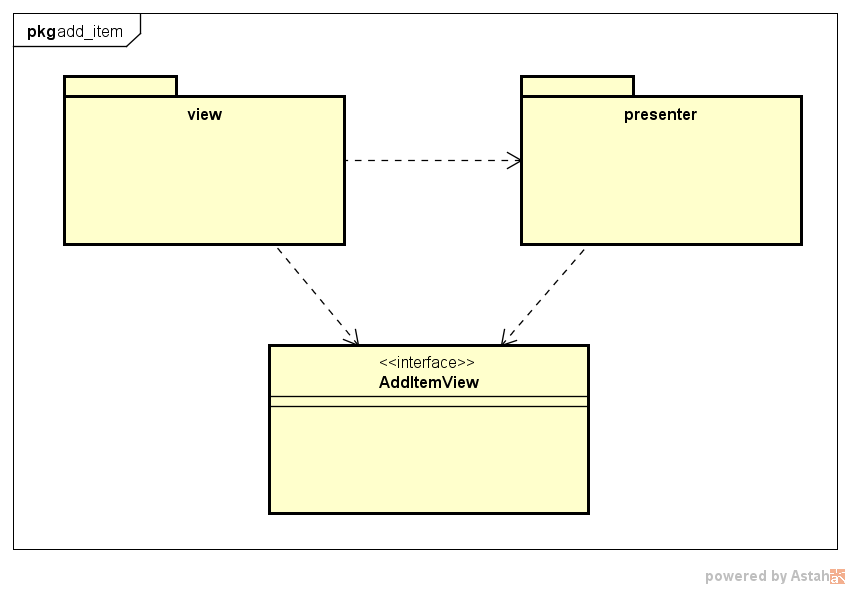
\includegraphics[scale=0.5]{Sezioni/Packages/App/add_item.png}
	\caption{Package application::feature::add\_item}
\end{figure}
\begin{itemize}
	\item \textbf{Descrizione}: package contenente i file relativi alla funzionalità di aggiunta elemento ad una lista
	\item \textbf{Classi e packages contenuti}:
	\begin{itemize}
	\item application::feature::add\_item::view: package contenente la view per l'aggiunta di un elemento
	\item application::feature::add\_item::presenter: package contenente il presenter per la view di aggiunta elemento
	\item application::feature::add\_item::AddItemView: interfaccia che rappresenta la vista di aggiunta oggetto
	\end{itemize}
\end{itemize}

\subsubsection{Package application::feature::add\_item::view}
\label{Package application::feature::add_item::view}
\begin{figure}[H]
	\centering
	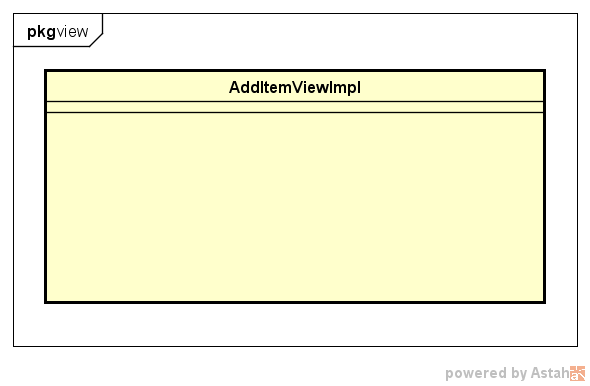
\includegraphics[scale=0.5]{Sezioni/Packages/App/add_item_view.png}
	\caption{Package application::feature::add\_item::view}
\end{figure}
\begin{itemize}
	\item \textbf{Descrizione}: package contenente la view per l'aggiunta di un elemento
	\item \textbf{Classi e packages contenuti}:
	\begin{itemize}
	\item application::feature::add\_item::view::AddItemViewImpl: implementazione dell'interfaccia AddItemView che rappresenta la vista di aggiunta di un oggetto alla lista
	\end{itemize}
\end{itemize}

\subsubsection{Package application::feature::add\_item::presenter}
\label{Package application::feature::add_item::presenter}
\begin{figure}[H]
	\centering
	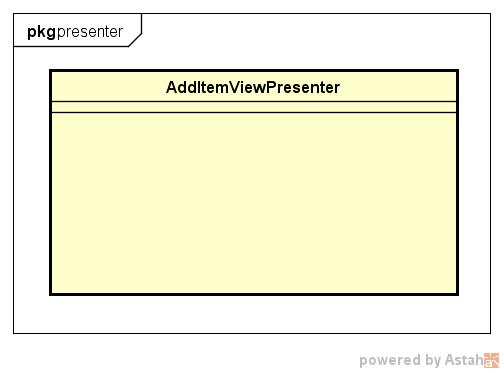
\includegraphics[scale=0.5]{Sezioni/Packages/App/add_item_presenter.png}
	\caption{Package application::feature::add\_item::presenter}
\end{figure}
\begin{itemize}
	\item \textbf{Descrizione}: package contenente il presenter per la vista di aggiunta di un oggetto alla lista
	\item \textbf{Classi e packages contenuti}:
	\begin{itemize}
	\item application::feature::add\_item::presenter::AddItemViewPresenter: presenter per la vista di aggiunta di un oggetto alla lista
	\end{itemize}
\end{itemize}

\subsubsection{Package application::feature::change\_list\_info}
\label{Package application::feature::change_list_info}
\begin{figure}[H]
	\centering
	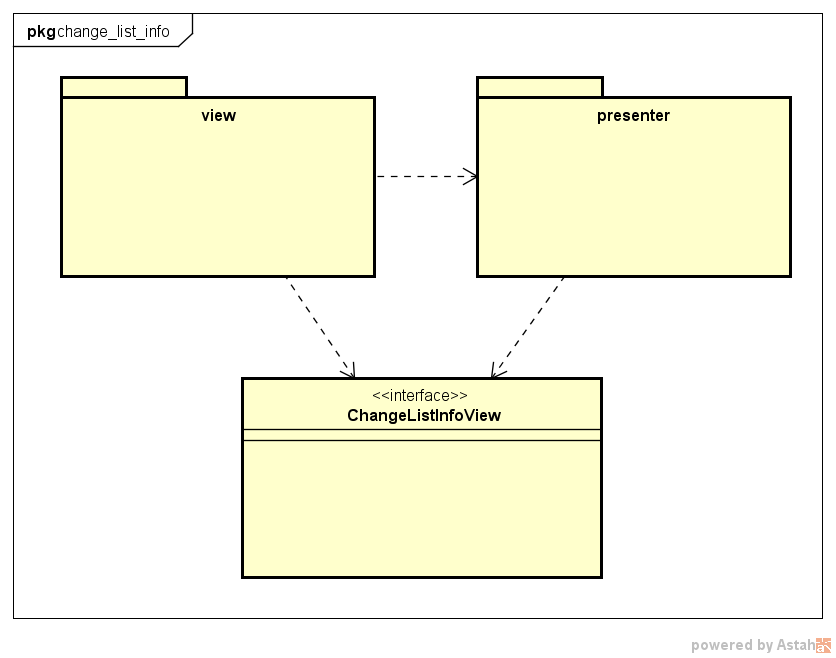
\includegraphics[scale=0.5]{Sezioni/Packages/App/change_list_info.png}
	\caption{Package application::feature::change\_list\_info}
\end{figure}
\begin{itemize}
	\item \textbf{Descrizione}: package contenente i componenti per la funzionalità di modifica informazioni di una lista
	\item \textbf{Classi e packages contenuti}:
	\begin{itemize}
	\item application::feature::change\_list\_info::view: package contenente la vista per la modifica informazioni di una lista
	\item application::feature::change\_list\_info::presenter: package contenente il presenter per la vista di modifica informazioni di una lista
	\item application::feature::change\_list\_info::ChangeListInfoView: interfaccia rappresentante la vista per la modifica informazioni di una lista
	\end{itemize}
\end{itemize}

\subsubsection{Package application::feature::change\_list\_info::view}
\label{Package application::feature::change_list_info::view}
\begin{figure}[H]
	\centering
	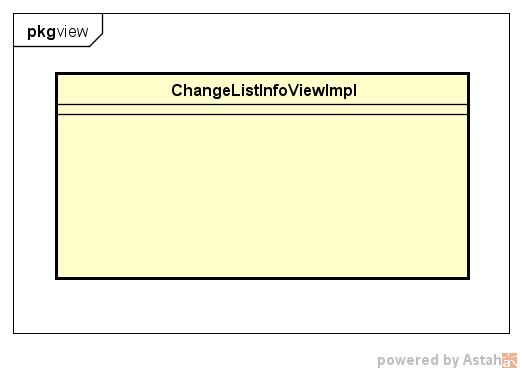
\includegraphics[scale=0.5]{Sezioni/Packages/App/change_list_info_view.png}
	\caption{Package application::feature::change\_list\_info::view}
\end{figure}
\begin{itemize}
	\item \textbf{Descrizione}: package contenente la vista per la funzionalità di modifica informazioni di una lista
	\item \textbf{Classi e packages contenuti}:
	\begin{itemize}
	\item application::feature::change\_list\_info::view::ChangeListInfoViewImpl: implementazione dell'interfaccia che rappresenta la vista per la funzionalità di modifica della informazioni di una lista
	\end{itemize}
\end{itemize}

\subsubsection{Package application::feature::change\_list\_info::presenter}
\label{Package application::feature::change_list_info::presenter}
\begin{figure}[H]
	\centering
	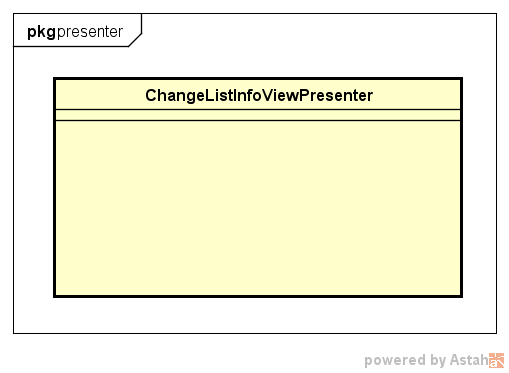
\includegraphics[scale=0.5]{Sezioni/Packages/App/change_list_info_presenter.png}
	\caption{Package application::feature::change\_list\_info::presenter}
\end{figure}
\begin{itemize}
	\item \textbf{Descrizione}: package contenente il presenter per la vista di modifica informazioni di una lista
	\item \textbf{Classi e packages contenuti}:
	\begin{itemize}
	\item application::feature::change\_list\_info::presenter::ChangeListInfoViewPresenter: classe che rappresenta il presenter per la vista di modifica dei dati di una lista
	\end{itemize}
\end{itemize}


\subsubsection{Package application::feature::create\_list}
\label{Package application::feature::create_list}
\begin{figure}[H]
	\centering
	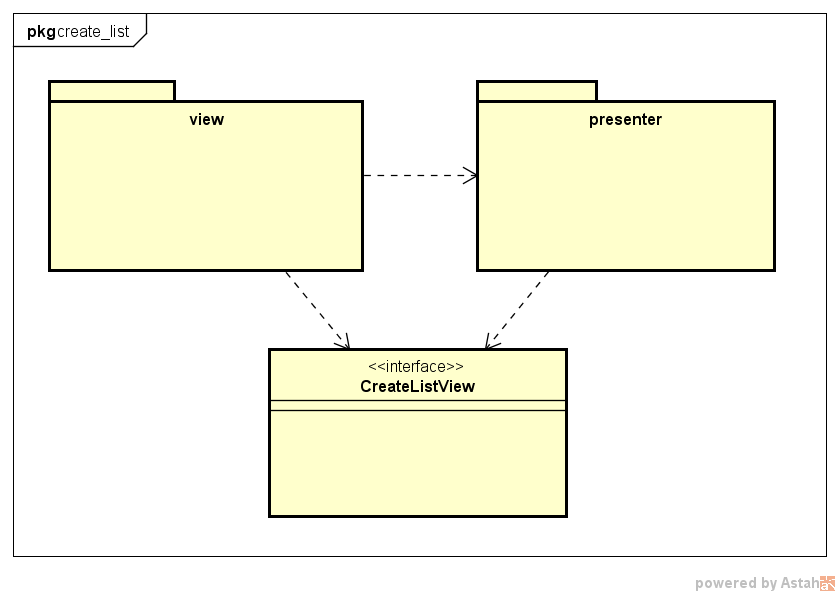
\includegraphics[scale=0.5]{Sezioni/Packages/App/create_list.png}
	\caption{Package application::feature::create\_list}
\end{figure}
\begin{itemize}
	\item \textbf{Descrizione}: package contenente i componenti per la funzionalità di creazione di una lista
	\item \textbf{Classi e packages contenuti}:
	\begin{itemize}
	\item application::feature::create\_list::view: package contenente la vista per la creazione di una lista
	\item application::feature::create\_list::presenter: package contenente il presenter per la vista di creazione di una lista
	\item application::feature::create\_list::CreateListView: interfaccia rappresentante la vista per la creazione di una lista
	\end{itemize}
\end{itemize}

\subsubsection{Package application::feature::create\_list::view}
\label{Package application::feature::create_list::view}
\begin{figure}[H]
	\centering
	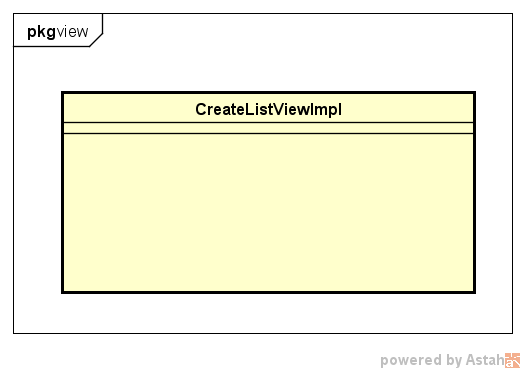
\includegraphics[scale=0.5]{Sezioni/Packages/App/create_list_view.png}
	\caption{Package application::feature::create\_list::view}
\end{figure}
\begin{itemize}
	\item \textbf{Descrizione}: package contenente la vista per la funzionalità di creazione di una lista
	\item \textbf{Classi e packages contenuti}:
	\begin{itemize}
	\item application::feature::create\_list::view::CreateListViewImpl: implementazione dell'interfaccia che rappresenta la vista per la funzionalità di creazione di una lista
	\end{itemize}
\end{itemize}

\subsubsection{Package application::feature::create\_list::presenter}
\label{Package application::feature::create_list::presenter}
\begin{figure}[H]
	\centering
	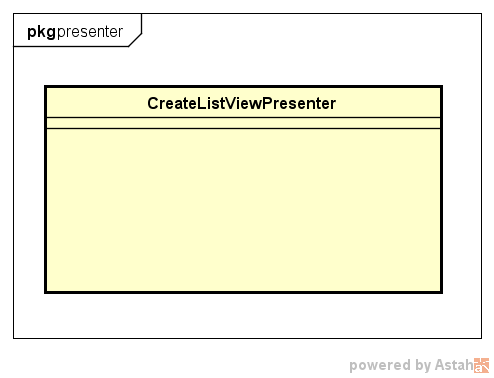
\includegraphics[scale=0.5]{Sezioni/Packages/App/create_list_presenter.png}
	\caption{Package application::feature::create\_list::presenter}
\end{figure}
\begin{itemize}
	\item \textbf{Descrizione}: package contenente il presenter per la vista di creazione di una lista
	\item \textbf{Classi e packages contenuti}:
	\begin{itemize}
	\item application::feature::create\_list::presenter::CreateListViewPresenter: classe che rappresenta il presenter per la vista di creazione di una lista
	\end{itemize}
\end{itemize}

\subsubsection{Package application::feature::forward}
\label{Package application::feature::forward}
\begin{figure}[H]
	\centering
	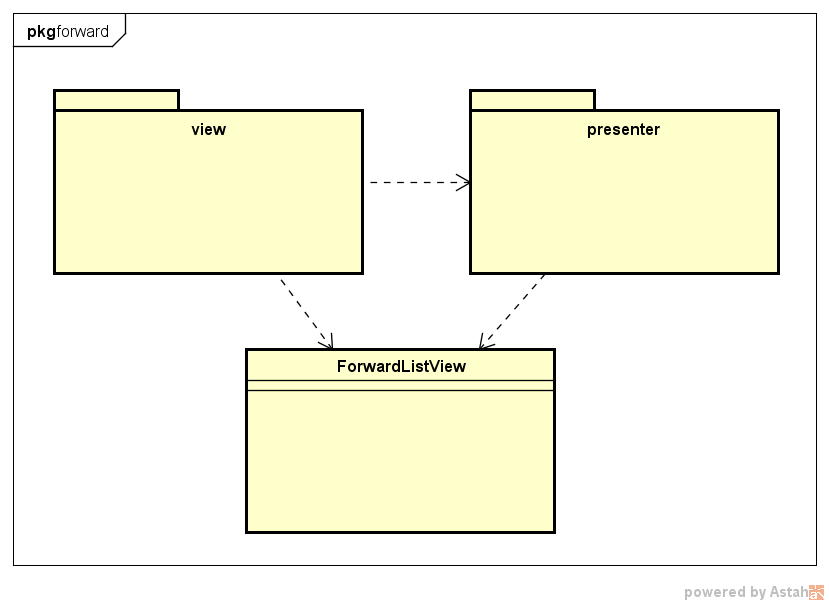
\includegraphics[scale=0.5]{Sezioni/Packages/App/forward.png}
	\caption{Package application::feature::forward}
\end{figure}
\begin{itemize}
	\item \textbf{Descrizione}: package contenente i componenti per la funzionalità di inoltro di una lista
	\item \textbf{Classi e packages contenuti}:
	\begin{itemize}
	\item application::feature::forward::view: package contenente la vista per la inoltro di una lista
	\item application::feature::forward::presenter: package contenente il presenter per la vista di inoltro di una lista
	\item application::feature::forward::ForwardListView: interfaccia rappresentante la vista per la funzionalità inoltro di una lista
	\end{itemize}
\end{itemize}

\subsubsection{Package application::feature::forward::view}
\label{Package application::feature::forward::view}
\begin{figure}[H]
	\centering
	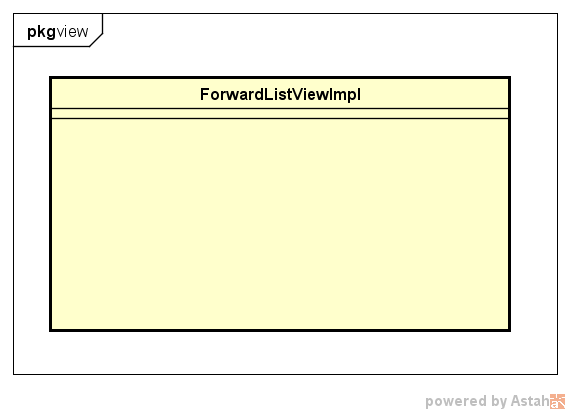
\includegraphics[scale=0.5]{Sezioni/Packages/App/forward_view.png}
	\caption{Package application::feature::forward::view}
\end{figure}
\begin{itemize}
	\item \textbf{Descrizione}: package contenente la vista per la funzionalità di inoltro di una lista
	\item \textbf{Classi e packages contenuti}:
	\begin{itemize}
	\item application::feature::forward::view::ForwardListViewImpl: implementazione dell'interfaccia che rappresenta la vista per la funzionalità di inoltro di una lista
	\end{itemize}
\end{itemize}

\subsubsection{Package application::feature::forward::presenter}
\label{Package application::feature::forward::presenter}
\begin{figure}[H]
	\centering
	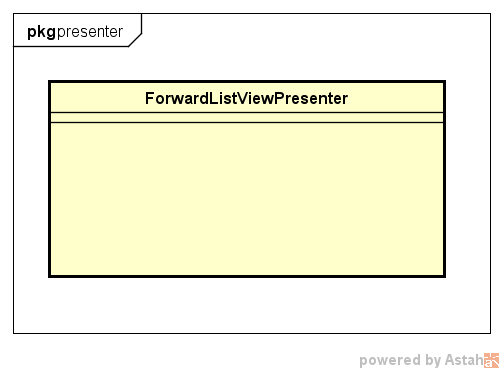
\includegraphics[scale=0.5]{Sezioni/Packages/App/forward_presenter.png}
	\caption{Package application::feature::forward::presenter}
\end{figure}
\begin{itemize}
	\item \textbf{Descrizione}: package contenente il presenter per la vista di inoltro di una lista
	\item \textbf{Classi e packages contenuti}:
	\begin{itemize}
	\item application::feature::forward::presenter::ForwardListViewPresenter: classe che rappresenta il presenter per la vista di inoltro di una lista
	\end{itemize}
\end{itemize}

\subsubsection{Package application::feature::input\_item\_info}
\label{Package application::feature::input_item_info}
\begin{figure}[H]
	\centering
	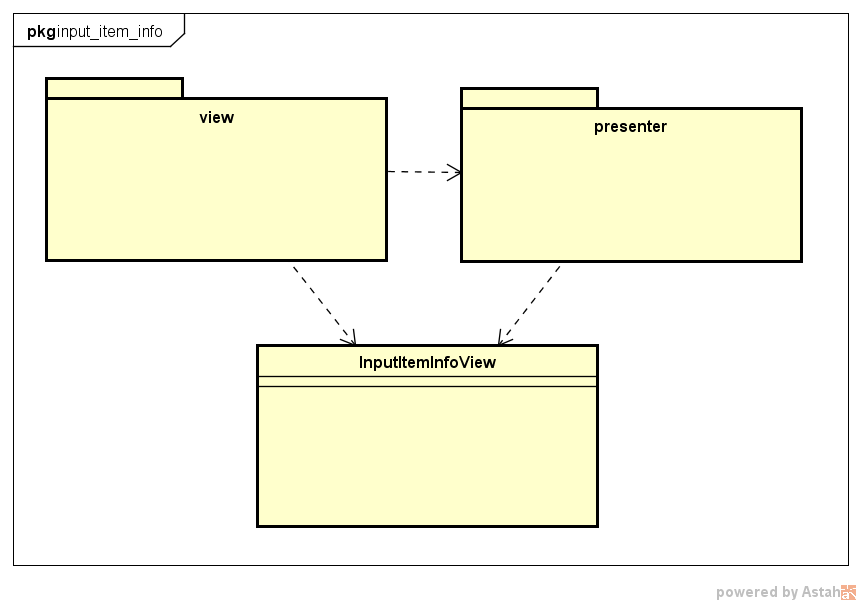
\includegraphics[scale=0.5]{Sezioni/Packages/App/input_item_info.png}
	\caption{Package application::feature::input\_item\_info}
\end{figure}
\begin{itemize}
	\item \textbf{Descrizione}: package contenente i componenti per la funzionalità di inserimento dati di un oggetto della lista
	\item \textbf{Classi e packages contenuti}:
	\begin{itemize}
	\item application::feature::input\_item\_info::view: package contenente la vista per la inserimento dati di un oggetto della lista
	\item application::feature::input\_item\_info::presenter: package contenente il presenter per la vista di inserimento dati di un oggetto della lista
	\item application::feature::input\_item\_info::InputItemInfoView: interfaccia rappresentante la vista per la funzionalità inserimento dati di un oggetto della lista
	\end{itemize}
\end{itemize}

\subsubsection{Package application::feature::input\_item\_info::view}
\label{Package application::feature::input_item_info::view}
\begin{figure}[H]
	\centering
	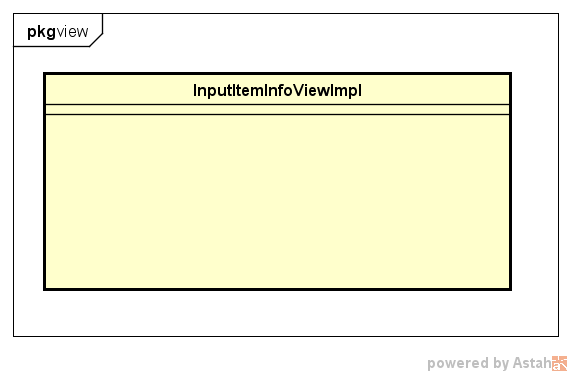
\includegraphics[scale=0.5]{Sezioni/Packages/App/input_item_info_view.png}
	\caption{Package application::feature::input\_item\_info::view}
\end{figure}
\begin{itemize}
	\item \textbf{Descrizione}: package contenente la vista per la funzionalità di inserimento dati di un oggetto della lista
	\item \textbf{Classi e packages contenuti}:
	\begin{itemize}
	\item application::feature::input\_item\_info::view::InputItemInfoViewImpl: implementazione dell'interfaccia che rappresenta la vista per la funzionalità di inserimento dati di un oggetto della lista
	\end{itemize}
\end{itemize}

\subsubsection{Package application::feature::input\_item\_info::presenter}
\label{Package application::feature::input_item_info::presenter}
\begin{figure}[H]
	\centering
	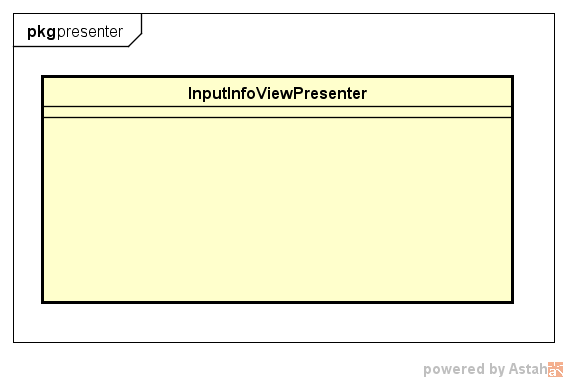
\includegraphics[scale=0.5]{Sezioni/Packages/App/input_item_info_presenter.png}
	\caption{Package application::feature::input\_item\_info::presenter}
\end{figure}
\begin{itemize}
	\item \textbf{Descrizione}: package contenente il presenter per la vista di inserimento dati di un oggetto della lista
	\item \textbf{Classi e packages contenuti}:
	\begin{itemize}
	\item application::feature::input\_item\_info::presenter::InputItemInfoViewPresenter: classe che rappresenta il presenter per la vista di inserimento dati di un oggetto della lista
	\end{itemize}
\end{itemize}


\subsubsection{Package application::feature::input\_list\_info}
\label{Package application::feature::input_list_info}
\begin{figure}[H]
	\centering
	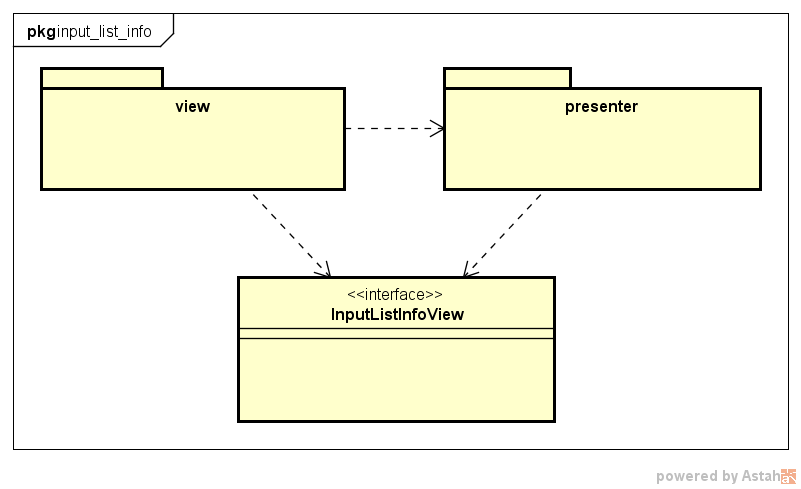
\includegraphics[scale=0.5]{Sezioni/Packages/App/input_list_info.png}
	\caption{Package application::feature::input\_list\_info}
\end{figure}
\begin{itemize}
	\item \textbf{Descrizione}: package contenente i componenti per la funzionalità di inserimento dati di una lista
	\item \textbf{Classi e packages contenuti}:
	\begin{itemize}
	\item application::feature::input\_list\_info::view: package contenente la vista per la inserimento dati di una lista
	\item application::feature::input\_list\_info::presenter: package contenente il presenter per la vista di inserimento dati di una lista
	\item application::feature::input\_list\_info::InputListInfoView: interfaccia rappresentante la vista per la funzionalità inserimento dati di una lista
	\end{itemize}
\end{itemize}

\subsubsection{Package application::feature::input\_list\_info::view}
\label{Package application::feature::input_list_info::view}
\begin{figure}[H]
	\centering
	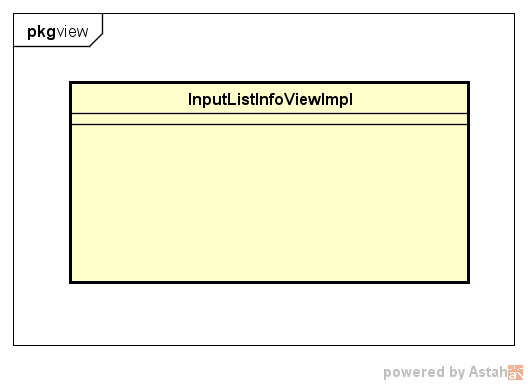
\includegraphics[scale=0.5]{Sezioni/Packages/App/input_list_info_view.png}
	\caption{Package application::feature::input\_list\_info::view}
\end{figure}
\begin{itemize}
	\item \textbf{Descrizione}: package contenente la vista per la funzionalità di inserimento dati di una lista
	\item \textbf{Classi e packages contenuti}:
	\begin{itemize}
	\item application::feature::input\_list\_info::view::InputListInfoViewImpl: implementazione dell'interfaccia che rappresenta la vista per la funzionalità di inserimento dati di una lista
	\end{itemize}
\end{itemize}

\subsubsection{Package application::feature::input\_list\_info::presenter}
\label{Package application::feature::input_list_info::presenter}
\begin{figure}[H]
	\centering
	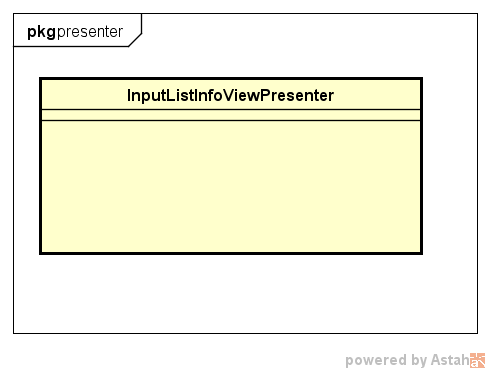
\includegraphics[scale=0.5]{Sezioni/Packages/App/input_list_info_presenter.png}
	\caption{Package application::feature::input\_list\_info::presenter}
\end{figure}
\begin{itemize}
	\item \textbf{Descrizione}: package contenente il presenter per la vista di inserimento dati di una lista
	\item \textbf{Classi e packages contenuti}:
	\begin{itemize}
	\item application::feature::input\_list\_info::presenter::InputListInfoViewPresenter: classe che rappresenta il presenter per la vista di inserimento dati di una lista
	\end{itemize}
\end{itemize}


\subsubsection{Package application::feature::modify\_item}
\label{Package application::feature::modify_item}
\begin{figure}[H]
	\centering
	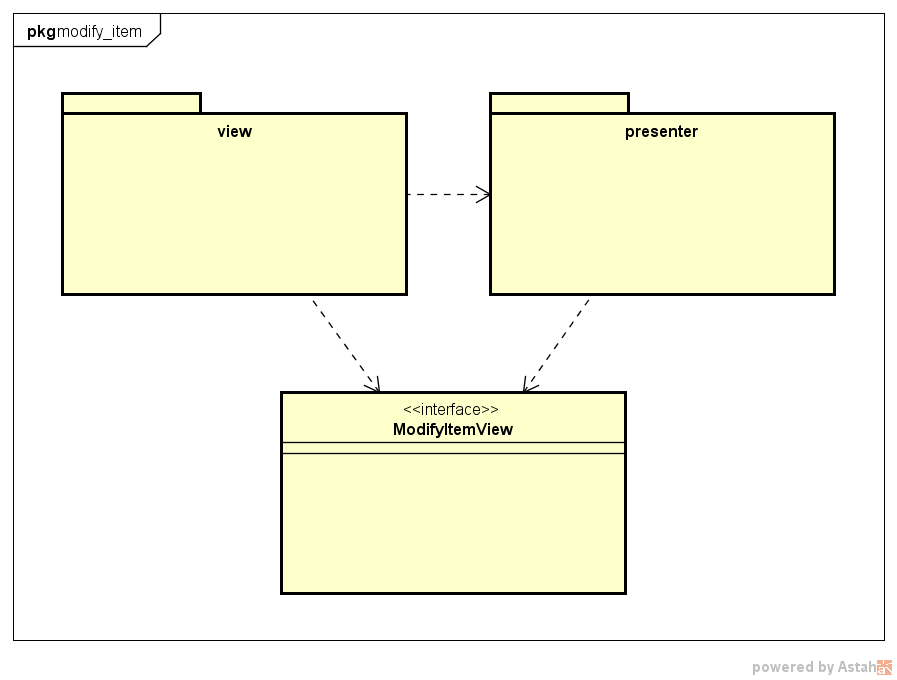
\includegraphics[scale=0.5]{Sezioni/Packages/App/modify_item.png}
	\caption{Package application::feature::modify\_item}
\end{figure}
\begin{itemize}
	\item \textbf{Descrizione}: package contenente i componenti per la funzionalità di modifica di un oggetto all'interno di una lista
	\item \textbf{Classi e packages contenuti}:
	\begin{itemize}
	\item application::feature::modify\_item::view: package contenente la vista per la modifica di un oggetto all'interno di una lista
	\item application::feature::modify\_item::presenter: package contenente il presenter per la vista di modifica di un oggetto all'interno di una lista
	\item application::feature::modify\_item::ModifyItemView: interfaccia rappresentante la vista per la funzionalità modifica di un oggetto all'interno di una lista
	\end{itemize}
\end{itemize}

\subsubsection{Package application::feature::modify\_item::view}
\label{Package application::feature::modify_item::view}
\begin{figure}[H]
	\centering
	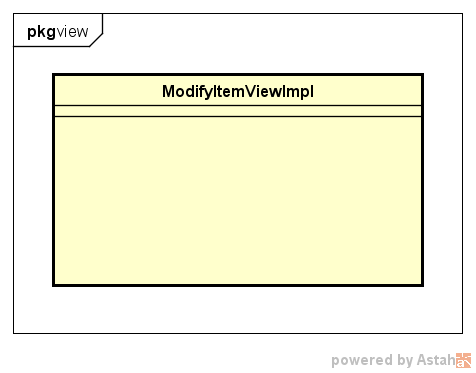
\includegraphics[scale=0.5]{Sezioni/Packages/App/modify_item_view.png}
	\caption{Package application::feature::modify\_item::view}
\end{figure}
\begin{itemize}
	\item \textbf{Descrizione}: package contenente la vista per la funzionalità di modifica di un oggetto all'interno di una lista
	\item \textbf{Classi e packages contenuti}:
	\begin{itemize}
	\item application::feature::modify\_item::view::ModifyItemViewImpl: implementazione dell'interfaccia che rappresenta la vista per la funzionalità di modifica di un oggetto all'interno di una lista
	\end{itemize}
\end{itemize}

\subsubsection{Package application::feature::modify\_item::presenter}
\label{Package application::feature::modify_item::presenter}
\begin{figure}[H]
	\centering
	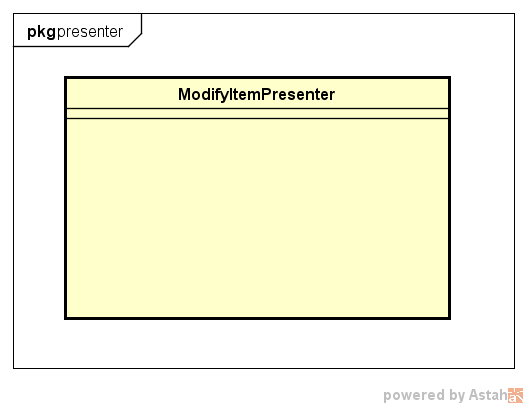
\includegraphics[scale=0.5]{Sezioni/Packages/App/modify_item_presenter.png}
	\caption{Package application::feature::modify\_item::presenter}
\end{figure}
\begin{itemize}
	\item \textbf{Descrizione}: package contenente il presenter per la vista di modifica di un oggetto all'interno di una lista
	\item \textbf{Classi e packages contenuti}:
	\begin{itemize}
	\item application::feature::modify\_item::presenter::ModifyItemViewPresenter: classe che rappresenta il presenter per la vista di modifica di un oggetto all'interno di una lista
	\end{itemize}
\end{itemize}


\subsubsection{Package application::feature::remove\_item}
\label{Package application::feature::remove_item}
\begin{figure}[H]
	\centering
	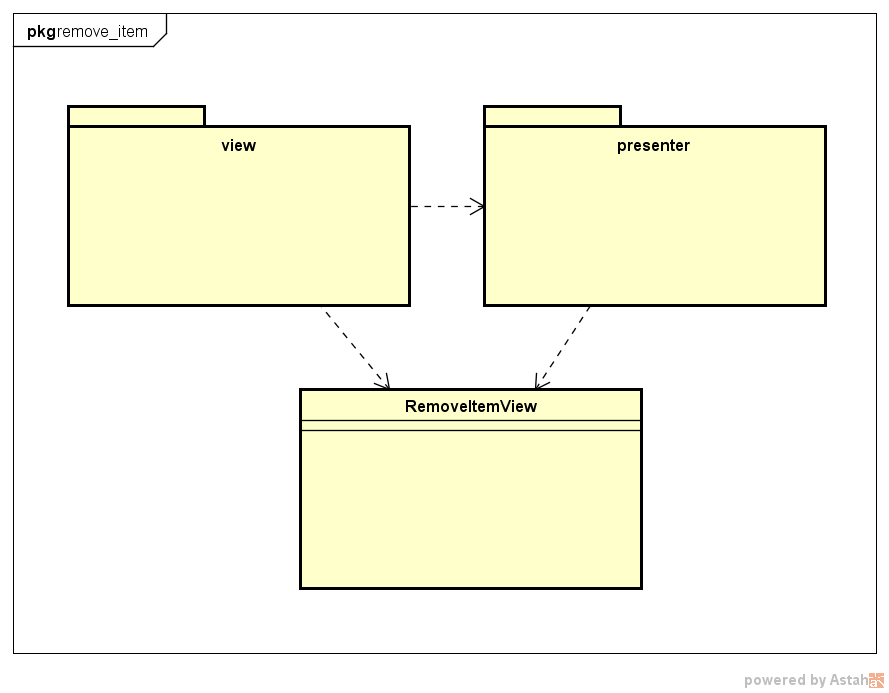
\includegraphics[scale=0.5]{Sezioni/Packages/App/remove_item.png}
	\caption{Package application::feature::remove\_item}
\end{figure}
\begin{itemize}
	\item \textbf{Descrizione}: package contenente i componenti per la funzionalità di rimozione di un oggetto da una lista
	\item \textbf{Classi e packages contenuti}:
	\begin{itemize}
	\item application::feature::remove\_item::view: package contenente la vista per la modifica di un oggetto all'interno di una lista
	\item application::feature::remove\_item::presenter: package contenente il presenter per la vista di modifica di un oggetto all'interno di una lista
	\item application::feature::remove\_item::RemoveItemView: interfaccia rappresentante la vista per la funzionalità modifica di un oggetto all'interno di una lista
	\end{itemize}
\end{itemize}

\subsubsection{Package application::feature::remove\_item::view}
\label{Package application::feature::remove_item::view}
\begin{figure}[H]
	\centering
	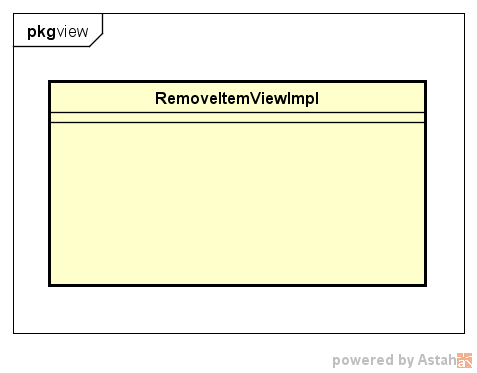
\includegraphics[scale=0.5]{Sezioni/Packages/App/remove_item_view.png}
	\caption{Package application::feature::remove\_item::view}
\end{figure}
\begin{itemize}
	\item \textbf{Descrizione}: package contenente la vista per la funzionalità di rimozione di un oggetto da una lista
	\item \textbf{Classi e packages contenuti}:
	\begin{itemize}
	\item application::feature::remove\_item::view::RemoveItemViewImpl: implementazione dell'interfaccia che rappresenta la vista per la funzionalità di rimozione di un oggetto da una lista
	\end{itemize}
\end{itemize}

\subsubsection{Package application::feature::remove\_item::presenter}
\label{Package application::feature::remove_item::presenter}
\begin{figure}[H]
	\centering
	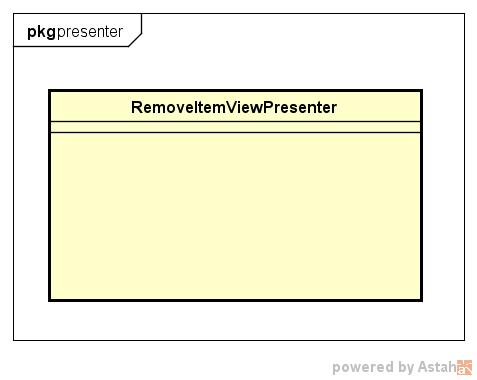
\includegraphics[scale=0.5]{Sezioni/Packages/App/remove_item_presenter.png}
	\caption{Package application::feature::forward::remove\_item::presenter}
\end{figure}
\begin{itemize}
	\item \textbf{Descrizione}: package contenente il presenter per la vista di rimozione di un oggetto da una lista
	\item \textbf{Classi e packages contenuti}:
	\begin{itemize}
	\item application::feature::remove\_item::presenter::RemoveItemViewPresenter: classe che rappresenta il presenter per la vista di rimozione di un oggetto da una lista
	\end{itemize}
\end{itemize}


\subsubsection{Package application::feature::sharewithcontact}
\label{Package application::feature::sharewithcontact}
\begin{figure}[H]
	\centering
	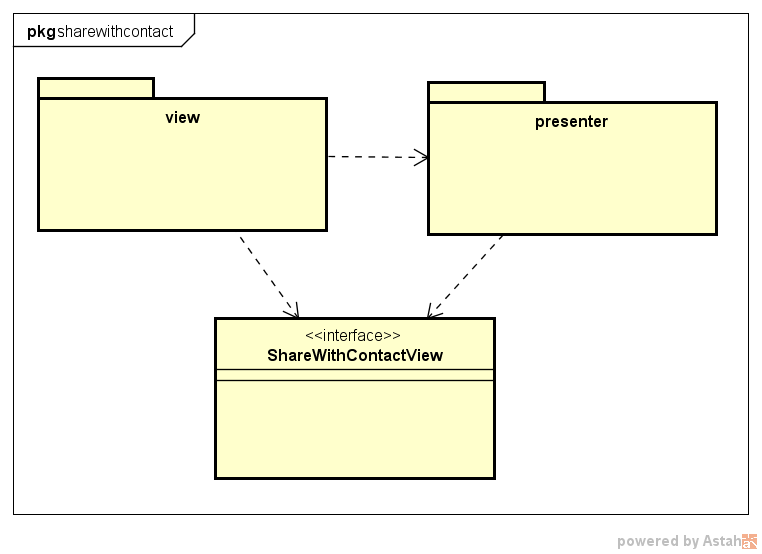
\includegraphics[scale=0.5]{Sezioni/Packages/App/share_with_contact.png}
	\caption{Package application::feature::sharewithcontact}
\end{figure}
\begin{itemize}
	\item \textbf{Descrizione}: package contenente i componenti per la funzionalità di condivisione della lista con un contatto
	\item \textbf{Classi e packages contenuti}:
	\begin{itemize}
	\item application::feature::sharewithcontact::view: package contenente la vista per la modifica di un oggetto all'interno di una lista
	\item application::feature::sharewithcontact::presenter: package contenente il presenter per la vista di modifica di un oggetto all'interno di una lista
	\item application::feature::sharewithcontact::ShareWithContactView: interfaccia rappresentante la vista per la funzionalità modifica di un oggetto all'interno di una lista
	\end{itemize}
\end{itemize}

\subsubsection{Package application::feature::sharewithcontact::view}\label{Package application::feature::sharewithcontact::view}
\begin{figure}[H]
	\centering
	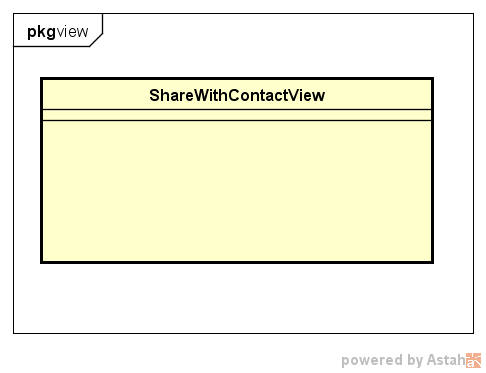
\includegraphics[scale=0.5]{Sezioni/Packages/App/share_with_contact_view.png}
	\caption{Package application::feature::sharewithcontact::view}
\end{figure}
\begin{itemize}
	\item \textbf{Descrizione}: package contenente la vista per la funzionalità di condivisione della lista con un contatto
	\item \textbf{Classi e packages contenuti}:
	\begin{itemize}
	\item application::feature::sharewithcontact::view::ShareWithContactViewImpl: implementazione dell'interfaccia che rappresenta la vista per la funzionalità di condivisione della lista con un contatto
	\end{itemize}
\end{itemize}

\subsubsection{Package application::feature::sharewithcontact::presenter}
\label{Package application::feature::sharewithcontact::presenter}
\begin{figure}[H]
	\centering
	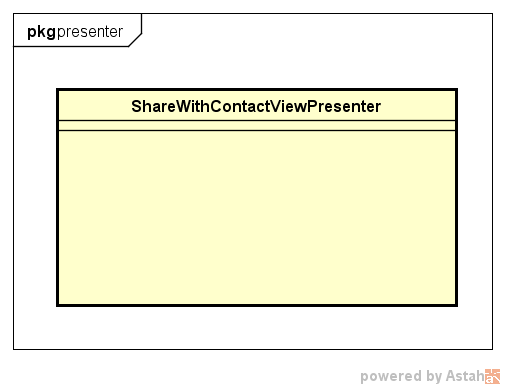
\includegraphics[scale=0.5]{Sezioni/Packages/App/share_with_contact_presenter.png}
	\caption{Package application::feature::sharewithcontact::presenter}
\end{figure}
\begin{itemize}
	\item \textbf{Descrizione}: package contenente il presenter per la vista di condivisione della lista con un contatto
	\item \textbf{Classi e packages contenuti}:
	\begin{itemize}
	\item application::feature::sharewithcontact::presenter::ShareWithContactViewPresenter: classe che rappresenta il presenter per la vista di condivisione della lista con un contatto
	\end{itemize}
\end{itemize}


\subsubsection{Package application::feature::sharewithgroup}
\label{Package application::feature::sharewithgroup}
\begin{figure}[H]
	\centering
	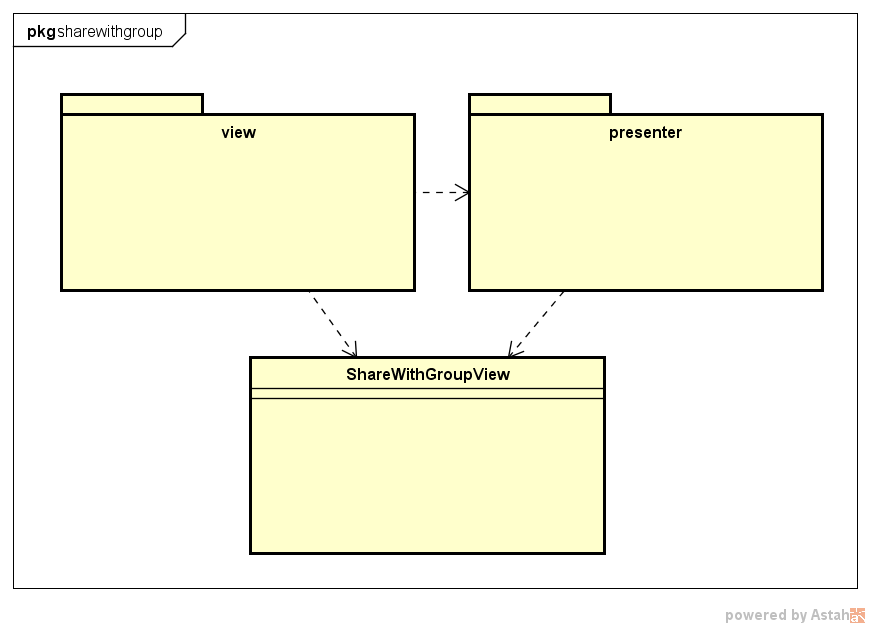
\includegraphics[scale=0.5]{Sezioni/Packages/App/share_with_group.png}
	\caption{Package application::feature::sharewithgroup}
\end{figure}
\begin{itemize}
	\item \textbf{Descrizione}: package contenente i componenti per la funzionalità di condivisione della lista con un gruppo
	\item \textbf{Classi e packages contenuti}:
	\begin{itemize}
	\item application::feature::sharewithgroup::view: package contenente la vista per la modifica di un oggetto all'interno di una lista
	\item application::feature::sharewithgroup::presenter: package contenente il presenter per la vista di modifica di un oggetto all'interno di una lista
	\item application::feature::sharewithgroup::ShareWithGroupView: interfaccia rappresentante la vista per la funzionalità modifica di un oggetto all'interno di una lista
	\end{itemize}
\end{itemize}

\subsubsection{Package application::feature::sharewithgroup::view}
\label{Package application::feature::sharewithgroup::view}
\begin{figure}[H]
	\centering
	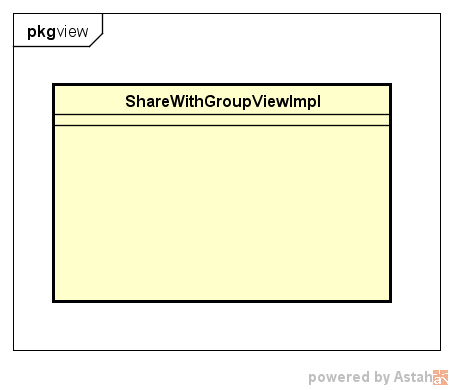
\includegraphics[scale=0.5]{Sezioni/Packages/App/share_with_group_view.png}
	\caption{Package application::feature::sharewithgroup::view}
\end{figure}
\begin{itemize}
	\item \textbf{Descrizione}: package contenente la vista per la funzionalità di condivisione della lista con un gruppo
	\item \textbf{Classi e packages contenuti}:
	\begin{itemize}
	\item application::feature::sharewithgroup::view::ShareWithGroupViewImpl: implementazione dell'interfaccia che rappresenta la vista per la funzionalità di condivisione della lista con un gruppo
	\end{itemize}
\end{itemize}

\subsubsection{Package application::feature::sharewithgroup::presenter}
\label{Package application::feature::sharewithgroup::presenter}
\begin{figure}[H]
	\centering
	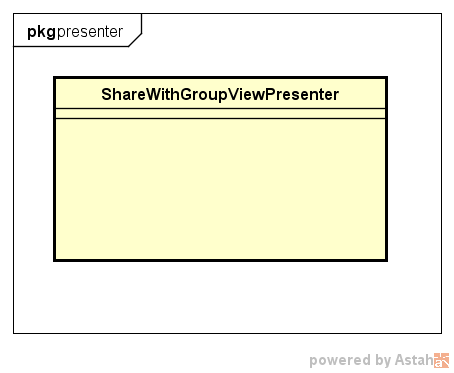
\includegraphics[scale=0.5]{Sezioni/Packages/App/share_with_group_presenter.png}
	\caption{Package application::feature::sharewithgroup::presenter}
\end{figure}
\begin{itemize}
	\item \textbf{Descrizione}: package contenente il presenter per la vista di condivisione della lista con un gruppo
	\item \textbf{Classi e packages contenuti}:
	\begin{itemize}
	\item application::feature::sharewithgroup::presenter::ShareWithGroupViewPresenter: classe che rappresenta il presenter per la vista di condivisione della lista con un gruppo
	\end{itemize}
\end{itemize}


\subsubsection{Package application::feature::help}
\label{Package application::feature::help}
\begin{figure}[H]
	\centering
	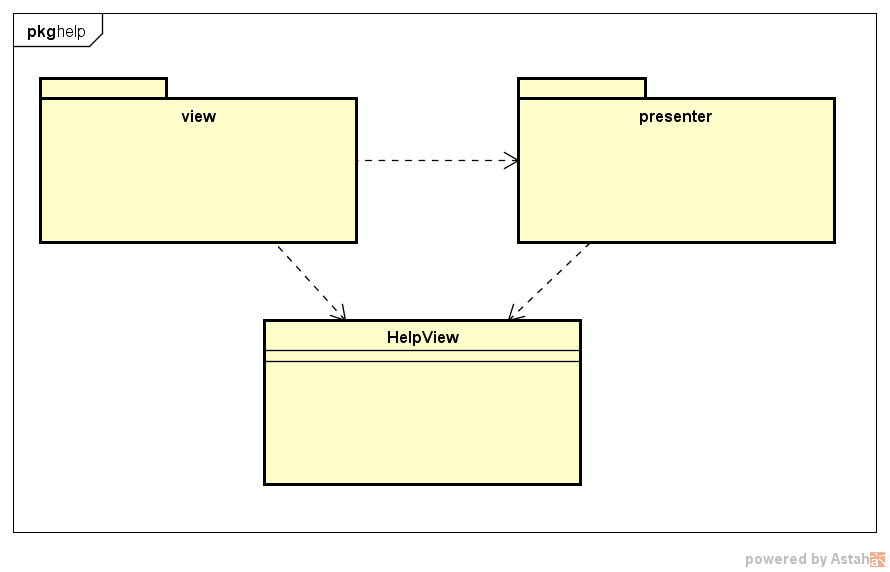
\includegraphics[scale=0.5]{Sezioni/Packages/App/help.png}
	\caption{Package application::feature::help}
\end{figure}
\begin{itemize}
	\item \textbf{Descrizione}: package contenente i componenti per la funzionalità di visualizzazione aiuto per l'utilizzo dell'applicazione
	\item \textbf{Classi e packages contenuti}:
	\begin{itemize}
	\item application::feature::help::view: package contenente la vista per la modifica di un oggetto all'interno di una lista
	\item application::feature::help::presenter: package contenente il presenter per la vista di modifica di un oggetto all'interno di una lista
	\item application::feature::help::helpView: interfaccia rappresentante la vista per la funzionalità modifica di un oggetto all'interno di una lista
	\end{itemize}
\end{itemize}

\subsubsection{Package application::feature::help::view}
\label{Package application::feature::help::view}
\begin{figure}[H]
	\centering
	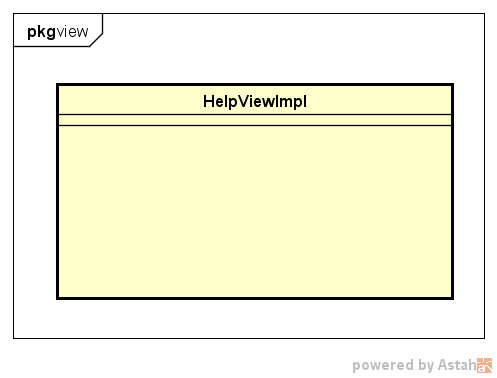
\includegraphics[scale=0.5]{Sezioni/Packages/App/help_view.png}
	\caption{Package application::feature::help::view}
\end{figure}
\begin{itemize}
	\item \textbf{Descrizione}: package contenente la vista per la funzionalità di visualizzazione aiuto per l'utilizzo dell'applicazione
	\item \textbf{Classi e packages contenuti}:
	\begin{itemize}
	\item application::feature::help::view::helpViewImpl: implementazione dell'interfaccia che rappresenta la vista per la funzionalità di visualizzazione aiuto per l'utilizzo dell'applicazione
	\end{itemize}
\end{itemize}

\subsubsection{Package application::feature::help::presenter}
\label{Package application::feature::help::presenter}
\begin{figure}[H]
	\centering
	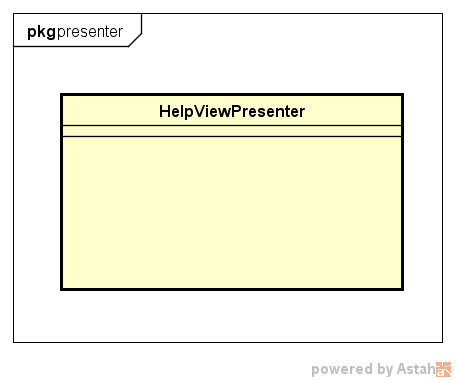
\includegraphics[scale=0.5]{Sezioni/Packages/App/help_presenter.png}
	\caption{Package application::feature::help::presenter}
\end{figure}
\begin{itemize}
	\item \textbf{Descrizione}: package contenente il presenter per la vista di visualizzazione aiuto per l'utilizzo dell'applicazione
	\item \textbf{Classi e packages contenuti}:
	\begin{itemize}
	\item application::feature::help::presenter::helpViewPresenter: classe che rappresenta il presenter per la vista di visualizzazione aiuto per l'utilizzo dell'applicazione
	\end{itemize}
\end{itemize}

\subsubsection{Package application::feature::exception}
\label{Package application::feature::exception}
\begin{figure}[H]
	\centering
	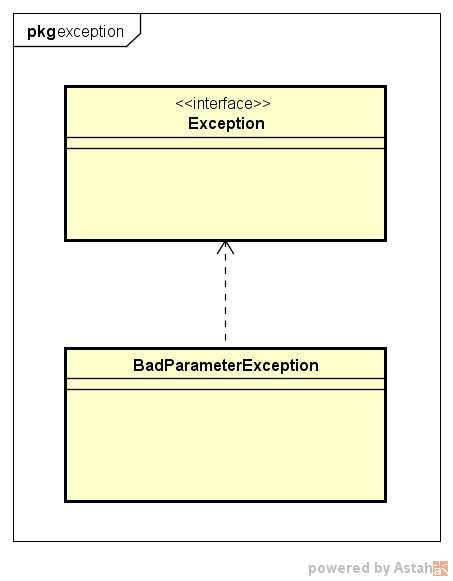
\includegraphics[scale=0.5]{Sezioni/Packages/App/exception.png}
	\caption{Package application::feature::exception}
\end{figure}
\begin{itemize}
	\item \textbf{Descrizione}: package contenente tutte le eccezioni che l'applicazione può lanciare durante l'esecuzione
	\item \textbf{Classi e packages contenuti}:
	\begin{itemize}
	\item application::feature::exception::Exception: classe che rappresenta una eccezione generica
	\item application::feature::exception::BadParameterException: classe che rappresenta una eccezione lanciata nel qual caso un parametro di un metodo sia incorretto
	\end{itemize}
\end{itemize}
\end{comment}